\chapter{Fundamentos Teóricos}
\label{chap:fundamentosteoricos}

Nesse presente capítulo será introduzido conceitos teóricos para a definição de axiomas e ferramentas do contexto. Será abordado primeiramente conceitos físicos no que tange a natureza do som como propagação, formação e dinâmica. Após será exposto fundamentos sobre notas musicais e harmonia. Enfim, então, será apresentado teorias computacionais de processamento de sinais e redes neurais de classificação.

\section{Conceitos Físicos do Som}
\label{sec:conceitosfiscossom}

O som pode ser visto como uma perturbação mecânica nas moléculas do meio, uma frente de compressão variável  de perfil mecânico e longitudinal com velocidade e pressão. O meio de propagação do som pode ser de diversas naturezas como por exemplo sólido, líquido e gasoso. Dessa perturbação mecânica entende-se como variação de pressão em relação ao tempo e espaço \cite{portela2008caracterizaccao}. Em vista disso, a equação diferencial que expressa o comportamento do som é a de natureza ondulatória $\textbf{p = p(x,t)}$:
\begin{equation}
\label{eqn01}
	\frac{\partial^{2}\mathbf{p}}{\partial x^{2}} = \frac{1}{c^{2}}\cdot \frac{\partial^{2}\mathbf{p}}{\partial t^{2}}
\end{equation} 

Na qual $\textbf{p}$ é a pressão, $\textbf{x}$ é a localização longitudinal, $\textbf{c}$ é a velocidade do som e $\textbf{t}$ é a localização temporal. A solução harmônica para a Equação (2.1) é definida por:  
\begin{equation}
\label{eqn02}
	\mathbf{p(x,t)} = \mathbf{A}.{exp}^{j(wt - kx)} + \mathbf{B}.{exp}^{j(wt + kx)}
\end{equation}

Em que $\textbf{k}$ é dado por $\textbf{w}/\textbf{c}$ e as constantes complexas $\textbf{A}$ e $\textbf{B}$ são utilizadas para condições de contorno.

Uma solução simples para a equação de onda 2.1 é a seguinte:
\begin{equation}
\label{eqn03}
	\mathbf{p(t)} = \mathbf{1}.{cos}(440.t)
\end{equation}

\newpage
Nela a variável $\textbf{x}$ foi fixada na origem do sistema cartesiano e o comportamento da onda só está sendo analisada em relação a variável temporal $\textbf{t}$. Há de considerar de suma importância a fixação frequencial $\textbf{w}$ em 440 Hz. Em termos musicais essa nota equivale ao Lá. Um exemplo de gráfico gerado por essa função é dado por:
\begin{figure}[h]
	\centering
		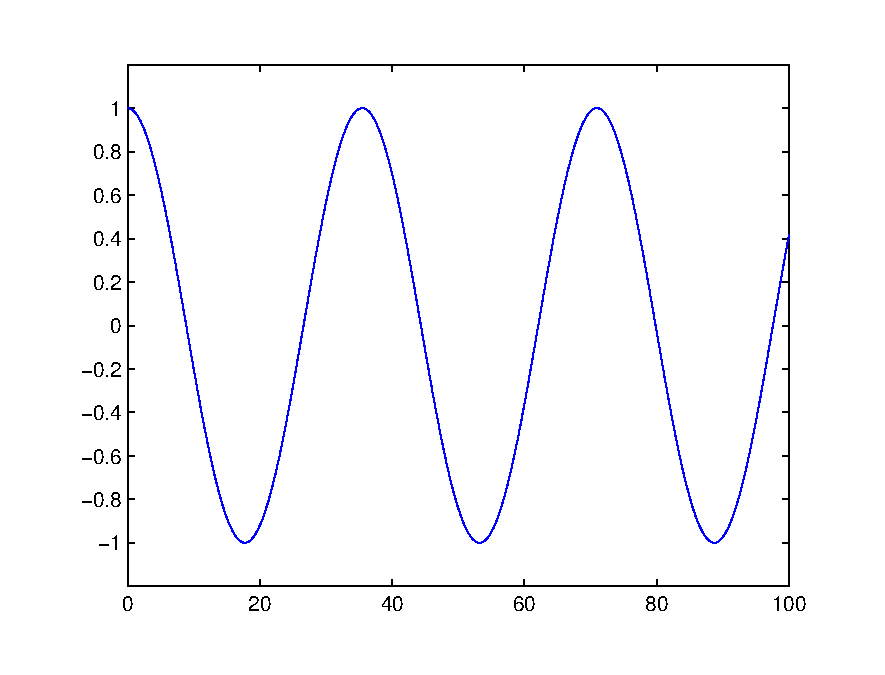
\includegraphics[scale=0.7]{figuras/cos440.eps}
	\caption{Função da Equação 2.3}
\end{figure}

Na forma mais teórica, um acorde, como será apresentado a seguir, é composto de no mínimo 3 ondas sonoras somadas, ou seja, para que seja formado um acorde Am por exemplo a equação total deverá ter essa forma: 
\begin{equation}
\label{eqn04}
	\mathbf{p(t)} = \mathbf{1}.{cos}(440.t) + \mathbf{0,5}.{cos}(523.t) + \mathbf{1}.{cos}(660.t)
\end{equation}

Pode-se considerar que cada constante multiplicadora das função cosseno determinará a energia de uma onda sonora específica. Nesse caso as ondas sonoras de mais energia são as de 440 Hz e 600 Hz. A onda de menor energia é a de 523 Hz que possui a metade da energia das outras. Esse fato será decisivo para a detecção de acordes. 

\newpage
Em termos de representação gráfica segue o resultado:
\begin{figure}[h]
	\centering
		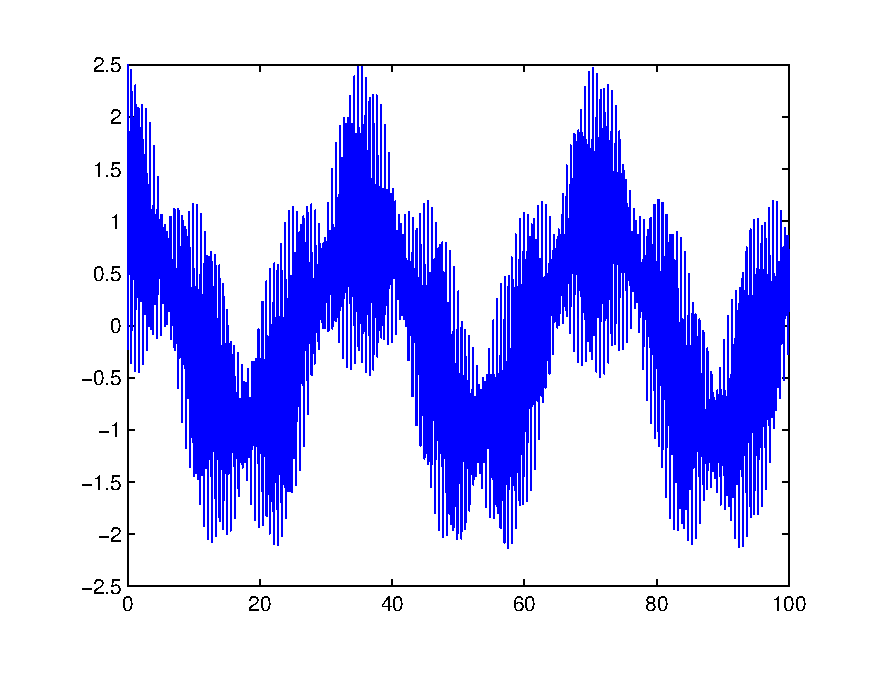
\includegraphics[scale=1]{figuras/Amcos.eps}
	\caption{Função da Equação 2.4}
\end{figure}

\section{Conceitos Musicais}
\label{sec:conceitosmusicais}

A música em si, além de ter em sua essência todas as leis físicas da ondulatória sonora, ela é uma forma de arte no que se refere a apresentação estética e do belo \cite{wolfflin2000conceitos}. Para a construção do belo em formas de som, há desenvolvido durante toda história da humanidade um conjunto de técnicas e metodologias bem apuradas. Nesse aspecto, a música defini-se como ciência e pode ser abordada nas áreas de teoria básica, solfejo, ritmo, percepção melódica, dinâmica, harmonia, contraponto, formas musicais, instrumentos musicais, instrumentação, orquestração, arranjo, fisiologia da voz, fonética, psicologia da música, pedagogia musical, história da música, acústica musical, análise musical, composição e regência \cite{med1996teoria}.

A estrutura da arte musical em si é baseada na combinação de sons em forma simultânea e sucessiva recorrendo a ordem, equilíbrio e proporção dentro do tempo. Os principais elementos formadores da música podem ser divididos nessas categorias:
\begin{itemize}
	\item melodia - sons dispostos em ordem sucessiva ao longo do tempo (concepção horizontal da música);
	\item harmonia - sons dispostos em ordem simultânea ao longo do tempo (concepção vertical da música);
	\item contraponto - conjunto de melodias e harmonias (concepção híbrida vertical e horizontal da música);
	\item ritmo - ordem e proporção em que estão dispostos as melodias e as harmonias.
\end{itemize}

O sons que formam as melodias e as harmonias possuem características principais como:
\begin{itemize}
	\item altura - frequência das vibrações sonoras. Quanto maior frequência mais agudo o som será;
	\item duração - tempo de extenção do som ao longo do tempo;
	\item intensidade - amplitudade ou força das vibrações sonoras, conhecido como volume;
	\item timbre - combinação das intensidades dos harmônicos que um determinado agente sonoro.
\end{itemize}

A altura e intensidade do som são as características essenciais para a formulação dos conceitos de notas e acordes. Em altura entende-se como a divisão das frequências em 7 notas musicas - $Dó$, $Ré$, $Mi$, $Fá$, $Sol$, $Lá$ e $Si$. Também essas mesmas notas possuem uma correspondente em sequência de letras alfabéticas introduzidas pelo Papa Gregório Grande - $C$, $D$, $E$, $F$, $G$, $A$ e $B$. Normalmente essa sequência de letras são usadas para denominar acordes. Entretanto tais divisões de notas não são a menor divisão para o sistema temperado \cite{med1996teoria}. A menor divisão de notas se denomina semitom e são configurados pelos acidentes sustenidos ($\#$) ou bemois ($\flat$). Considerando essa divisão semitonal o sistema fica representado nessa sequência de 12 notas musicais (entre uma divisão e outra há a presença de um semitom): $Dó$, $Dó\#$ ou $Ré\flat$, $Ré$, $Ré\#$ ou $Mi\flat$, $Mi$, $Fá$, $Fá\#$ ou $Sol\flat$, $Sol$, $Sol\#$ ou $Lá\flat$, $Lá$, $Lá\#$ ou $Si\flat$ e $Si$. Ou seguindo a denominação inglesa: $C$, $C\#$ ou $D\flat$, $D$, $D\#$ ou $E\flat$, $E$, $F$, $F\#$ ou $G\flat$, $G$, $G\#$ ou $A\flat$, $A$, $A\#$ ou $B\flat$ e $B$.

\newpage
Na divisão distributiva das faixas de frequências pelas notas segue um quadro básico \cite{notasfreq}: 
\begin{figure}[h]
	\centering
		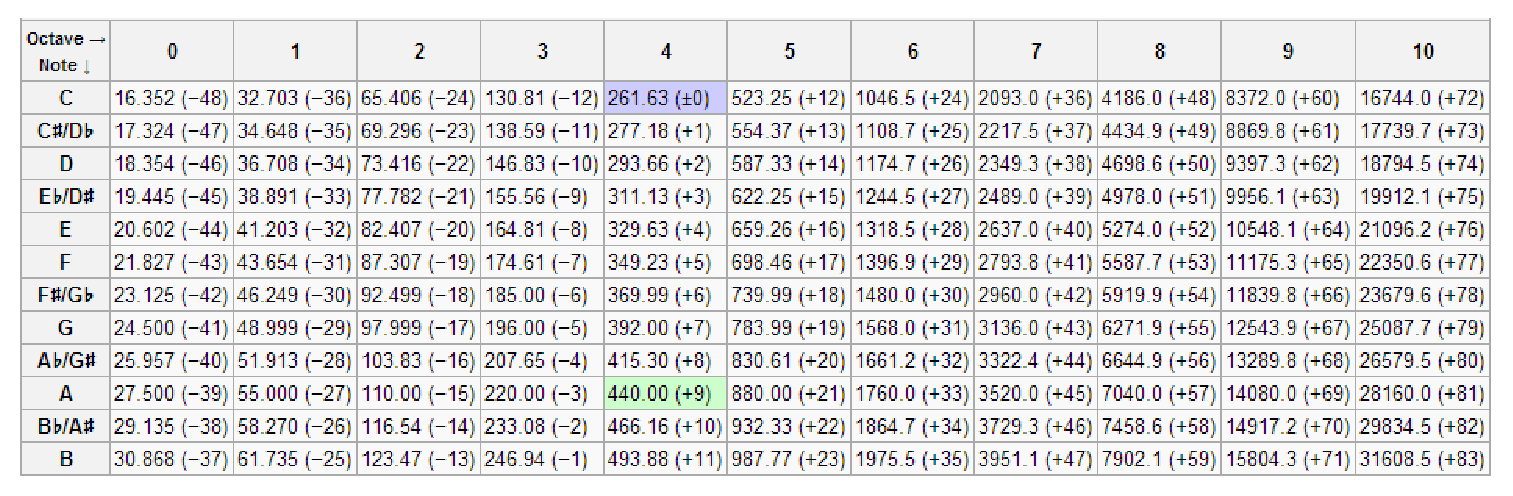
\includegraphics[scale=0.6]{figuras/NOTASpt.eps}
	\caption{Distribuição das frequências nas notas musicais em Hz}
\end{figure}    

Acordes são harmonias formadas por pelo menos uma tríade (três notas)\footnote{Existem acordes mais complexos com mais de 3 notas porém o escopo desse trabalho só se delimita a tríades.} tocadas simultâneamente e são definidos por certas quantidades de semitons entre as notas \cite{med1996teoria}. Essa quantidade se denomina intervalo musical.

As 3 notas da tríade são referenciadas como tônica (a nota base do acorde), terça e quinta \cite{med1996teoria}. Para acordes maiores ($M$) a distância entre a tônica e a terça é de 4 semitons (terça maior) e entre a tônica e a quinta é de 7 semitons (quinta justa). Para acordes menores ($m$) a distância entre a tônica e a terça é de 3 semitons (terça menor) e entre a tônica e a quinta é de 7 semitons (quinta justa). Para acordes aumentados ($aum$) a distância entre a tônica e a terça é de 4 semitons (terça maior) e entre a tônica e a quinta é de 8 semitons (quinta aumentada). Para acordes diminutos ($dim$) a distância entre a tônica e a terça é de 3 semitons (terça menor) e entre a tônica e a quinta é de 6 semitons (quinta diminuta).

Exemplos de acordes maiores são:
\begin{itemize}
	\item dó maior - $CM$ (tríade $Dó$, $Mi$ e $Sol$);
	\item lá maior - $AM$ (tríade $Lá$, $Dó\#$ e $Mi$).
\end{itemize}

Exemplos de acordes menores são:
\begin{itemize}
	\item mi menor - $Em$ (tríade  $Mi$, $Sol$ e $Si$,);
	\item ré sustenido menor - $D\#m$ (tríade $Ré\#$, $Fá\#$ e $Lá\#$).
\end{itemize}

Exemplos de acordes aumentados são:
\begin{itemize}
	\item sol aumentado - $Gaum$ (tríade  $Sol$, $Si$ e $Ré\#$);
	\item si aumentado - $Baum$ (tríade $Si$, $Ré\#$ e $Sol$).
\end{itemize}

Exemplos de acordes diminutos são:
\begin{itemize}
	\item dó sustenido diminuto - $C\#dim$ (tríade $Dó\#$, $Mi$ e $Sol$);
	\item lá sustenido diminuto - $A\#dim$ (tríade $Lá\#$, $Dó\#$ e $Mi$).
\end{itemize}

Na teoria dos acordes também há a presença do conceito de inversões. Inverter um acorde consiste em trocar de posição para uma oitava a cima a nota inferior, trocar a nota mais baixa do acorde por uma outra da mesma denominação só que com o dobro de frequência acima. Em tríades há a presença do acorde em seu estado fundamental, a primeira inversão (a terça fica sendo como a nota mais grave) e a segunda inversão (a quinta fica sendo como a nota mais grave).

Segue exemplos de acordes em estado fundamental: 
\begin{itemize}
	\item dó maior - $CM$ (tríade $Dó$, $Mi$ e $Sol$);
	\item mi menor - $Em$ (tríade  $Mi$, $Sol$ e $Si$,);
	\item sol aumentado - $Gaum$ (tríade  $Sol$, $Si$ e $Ré\#$);
	\item lá sustenido diminuto - $A\#dim$ (tríade $Lá\#$, $Dó\#$ e $Mi$).
\end{itemize}

Segue exemplos de acordes em primeira inversão: 
\begin{itemize}
	\item dó maior - $CM$ (tríade $Mi$, $Sol$ e $Dó$);
	\item mi menor - $Em$ (tríade $Sol$, $Si$ e $Mi$);
	\item sol aumentado - $Gaum$ (tríade $Si$, $Ré\#$ e $Sol$);
	\item lá sustenido diminuto - $A\#dim$ (tríade $Dó\#$, $Mi$ e $Lá\#$).
\end{itemize}

Segue exemplos de acordes em segunda inversão: 
\begin{itemize}
	\item dó maior - $CM$ (tríade $Sol$, $Dó$ e $Mi$);
	\item mi menor - $Em$ (tríade $Si$, $Mi$ e $Sol$);
	\item sol aumentado - $Gaum$ (tríade $Ré\#$, $Sol$ e $Si$);
	\item lá sustenido diminuto - $A\#dim$ (tríade $Mi$, $Lá\#$ e $Dó\#$).
\end{itemize}

\section{Conceitos de Processamento de Sinais}
\label{sec:conceitosprocessamentosinais}
%sinal o que é
O conceito de processamento de sinais está inteiramente ligado a natureza do sinal e a aplicação que normalmente se dá é de modificação ou análise. Sinal pode ser entendido como um objeto matemático, normalmente uma função matemática, que descreve o comportamento de um determinado fenômeno da natureza podendo ser, entre outros, físico, químico, biológico e financeiro \cite{oppenheim}.

Da natureza do sinal abordado, é explícito de que o mesmo é de cunho físico - sinais sonoros. Com a possibilidade de se trabalhar com sinal sonoro, há em processamento de sinais a liberdade de modificar ou extrair informações relevatantes para uma dada aplicação. Nesse contexto o sinal será processado com o intuito de colher informações para serem analisadas de forma a deduzir comportamentos de ondas sonoras.

Os sinais geralmente são funções relacionadas ao tempo. Eles podem ser processados em tempo contínuo (analogicamente) ou em tempo discreto (digitalmente). O escopo desse trabalho está restringido somente ao processamento na forma digital.

%amostragem e quantização
Para haver processamento digital é preciso que o sinal seja descrito computacionalmente num hardware. A forma de captação de um fenômeno contínuo para o ambiente computacional se denomina processo de amostragem e quantização \cite{amostragem}.

Amostrar um sinal significa recolher um número determinado de amostras dado um período de tempo, ou seja, haverá uma frequência (taxa de amostragem) \textbf{F} associada a um período de tempo \textbf{T} que proporcionará um conjundo finito de amostras num intervalo temporal. A relação exposta dar-se-à por:
\begin{equation}
\label{eqn05}
	\mathbf{F_s} = \frac{1}{T}
\end{equation}

Segundo o teorema de amostragem Nyquist–Shannon \cite{Nyquist}, para sons musicais o mais adequado é que a taxa de amostragem seja o dobro da frequência máxima de audição do ouvido humano - 22.050 Hz, ou seja, a frequência será de 44.100 Hz. Essa grandeza significa que serão captadas 44.100 amostras de áudio a cada segundo.

Quantizar um sinal significa alocar valores digitais para os valores analógicos do eixo da ordenada, que são normalmente valores de tenões elétricas. Essa a alocação está ligada diretamente as características do conversor analógico/digital. Nesse caso específico foi usado um conversor de 16 bits para a quantização do sinal. Tal fato permite a presença de 65.536 (2 elevado a 16) valores para representar as subidas e descidas da onda sonora.    

%energia
O conceito de energia está totalmente ligado a muitas outras áreas e é de extrema importância por ser essencial nos fenômenos naturais \cite{oppenheim}. Em processamento de sinais há a descrição de energia e dar-se-à pela fórmula em tempo contínuo num intervalo \textbf{$t1$} a \textbf{$t2$}: 
\begin{equation}
\label{eqn06}
	\mathbf{E} = \int_{t1}^{t2}{|x_c(t)|^{2}dt}
\end{equation}

O aspecto energético adotado nessa presente solução será em tempo discreto que é definido como:
\begin{equation}
\label{eqn07}
	\mathbf{E} = \sum_{t=t1}^{t2}{|x[n]|^{2}} 
\end{equation}

Outro conceito relacionado que é de extrema importância é a lei de conservação de energia representada pelo teorema de Parseval. Esse teorema mostra que a energia do sinal sempre se conserva independentemente da projeção que o sinal foi submetido. Mais especificamente na transformada de fourier no domínio contínuo o teorema é descrito como:  
\begin{equation}
\label{eqn08}
	\int_{-\infty}^{\infty}{|x(t)|^{2}dt} = \int_{-\infty}^{\infty}{|X(f)|^{2}df}
\end{equation}

Tal qual $X(f)$ é a transformada de fourier do sinal (exposto logo a seguir).
A mesma representação em tempo e frequência discretos é formada por:
\begin{equation}
\label{eqn09}
	\sum_{n=0}^{N - 1}{|x[n]|^{2}} =  \frac{1}{N}.\sum_{k=0}^{N - 1}{|X[k]|^{2}}
\end{equation}
Tal qual $N$ é o número total de amostras e $X(k)$ a transformada discreta de fourier.

%transformada de fourier
A transformada de fourier é uma ferramenta muito importante para a realização desse trabalho. Ela permite projetar o sinal em funções de base senoidais, ou seja, é possível ver através dela quais componentes frequenciais de senóides estão presentes no sinal e qual é a energia das mesmas.

A representação da transformada de fourier no domínio contínuo é dada por:
\begin{equation}
\label{eqn10}
	X(f) = \int_{-\infty}^{\infty}{x_c(t).{exp}^{-j2\pi.ft}dt}
\end{equation}
Tal qual $X(f)$ é a transformada de fourier contínua.

A representação da transformada inversa de fourier no domínio contínuo é dada por:
\begin{equation}
\label{eqn11}
	x_c(t) = \int_{-\infty}^{\infty}{X(f).{exp}^{j2\pi.ft}df}
\end{equation}

A representação da transformada de fourier em tempo e frequência discretos (DFT) é dada por:
\begin{equation}
\label{eqn12}
	X[k] = \sum_{n=0}^{N - 1}{x[n].{exp}^{-j2\pi.\frac{k}{N}.t}}
\end{equation}

A representação da transformada inversa de fourier em tempo e frequência discretos é dada por:
\begin{equation}
\label{eqn13}
	x[n] = \sum_{k=0}^{N - 1}{X[k].{exp}^{j2\pi.\frac{k}{N}.t}}
\end{equation}


\section{Conceitos de Redes Neurais Artificiais}
\label{sec:conceitosredesneurais}

Identificar padrões num sinal nem sempre é um trabalho trivial ou até mesmo determinístico. Normalmente sinais possuem ruídos intratáveis, sua composição é complexa no sentido de haver muitas amostras para análise e, como os sinais são fenômenos naturais, facilmente são vistos como sistemas complexos \cite{morin}. Determinar uma equação ou um algorítmo fixo e determinístico para classificação e processamento de sinais é bastante limitado e aderente há vários erros.

Diante desse ambiente de incertezas, uma solução que é aderente ao contexto é o uso de redes neurais artificiais. Essa técnica, além de prover as características necessárias para deixar a solução estável, ela modela o funcionamento neural de organismos vivos. Esse fato é muito interessante visto que surge a possibilidade de usar os mesmos mecanismos (de forma análoga) de reconhecimento de padrões sonoros do cérebro humano num sistema computacional.

Dado um especialista que possui o reconhecimento de padrões dos acordes, basta somente consolidar uma arquitetura de rede neural para receber esse conhecimento empírico de modo que o seu uso seja eficiente para classificação.

Entende-se por rede neural como ``um processador maciçamente paralelamente distribuído constituído de unidades de processamento simples, que têm a propensão para armazenar conhecimento experimental e torná-lo disponível para o uso'' \cite{haykin2009neural}. 

As redes neurais possuem uma característica essencial no que tange o aprendizado empírico. Sua estrutura oferece suporte para que conhecimentos adquiridos de maneira experimental (via ser humano muitas vezes) possam ser aprendidos e usados. O processo de aprendizagem da rede se chama algorítmo de aprendizado e o mesmo pode ser feito de várias formas como lei de Hebb, algorítmo de $backpropagation$, estratégias de competição e máquina de Boltzmann. Além disso é envolvido nesse processo paradígmas de aprendizado que é como o ambiente vai atuar sobre a rede neural para que ela possa aprender. Exemplos de paradígmas de aprendizado são aprendizado supervisionado, aprendizado por reforço e aprendizado não-supervisionado (ou auto-organizado).

Outra característica essencial de uma rede neural é a representação do conhecimento. Essa característica é referente às informações armazenadas ou a modelos utilizados por uma pessoa ou máquina com o intuito de interpretar, prever e responder de forma coerente ao mundo exterior \cite{haykin2009neural}. Para tal representação deve-se levantar em conta quais informações serão abstraídas e tornadas explícitas e como a informação será codificada no sistema. Com o intuito de atingir os objetivos de uma boa representação do conhecimento na rede neural há um conjunto de regras sugeridas a se seguir \cite{haykin2009neural}: 
\begin{itemize}
	\item regra 1 - entradas similares normalmente devem produzir representações similares no interior da rede e devem ser classificadas como pertencentes a mesma categoria;
	\item regra 2 - itens de classes diferentes devem ser representados de formas diferentes;
	\item regra 3 - se uma característica é importante deve-se haver um grande número de neurônios envolvidos na representação daquele item de rede;
	\item regra 4 - informações prévias e invariâncias devem ser incorporadas a rede para que o sistema fique simples e sem trabalho para aprender as mesmas.
\end{itemize}

Por fim outra característica importante de uma rede neural é a capacidade de generalização. Isso permite com que entradas desconhecidas possam ser classificadas e tratadas de forma coesa e coerente, fazendo com que circunstâncias críticas e imprevisíveis possam ser contornadas sem grandes prejuízos. 

A unidade mínima de processamento de uma rede neural é o neurônio artificial. Segue uma representação de um modelo \cite{haykin2009neural}: 

\begin{figure}[h]
	\centering
		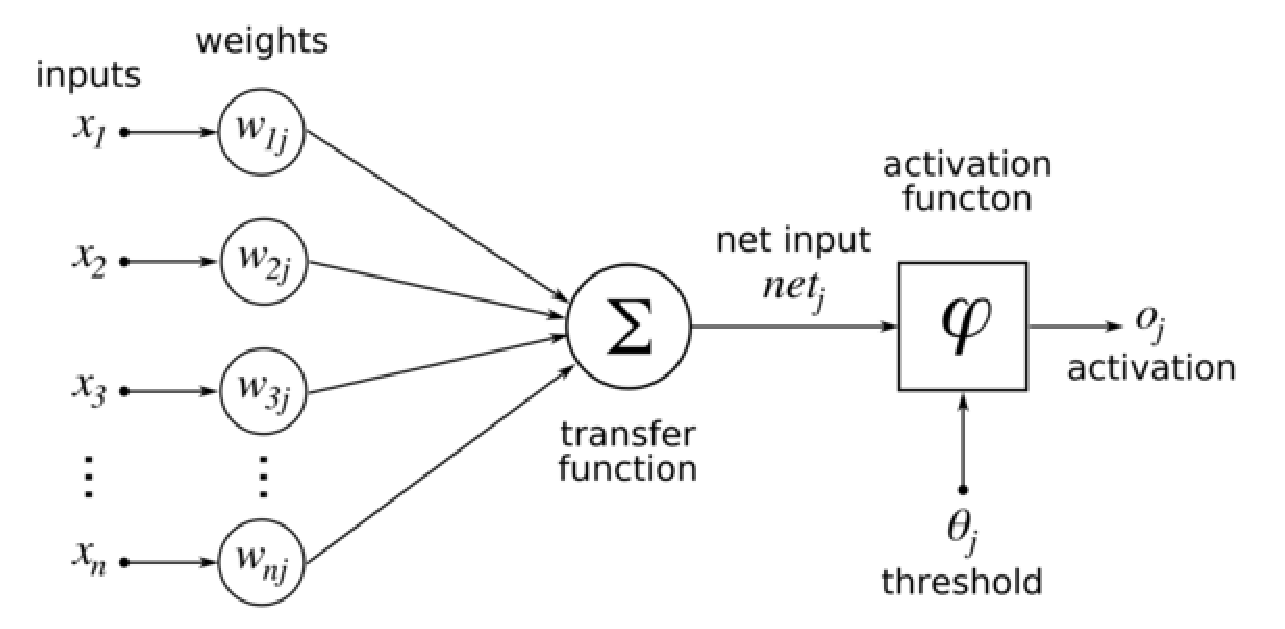
\includegraphics[scale=0.7]{figuras/neuron.eps}
	\caption{Modelo de um neurônio}
\end{figure}

Como é representado na figura os conjuntos de $w$ representam pesos sinápticos para a modulação dos sinais de entrada. Após há um somador para efetuar operações de combinações lineares. Por último há uma função de ativação, mais conhecido como um limiar de ativação para que a resposta possa ser propagada a outros neurônios.

\newpage
Para o presente problema, foi sugerido o uso da rede neural do tipo PNN (Probabilistic Neural Network). Ela é inerentemente um sistema de classificação bastante simples de aprendizado não-supervisionado, ou seja, novos conhecimentos são adquiridos pela simples inserção de novos neurônios. Segue o modelo arquitetural \cite{neuron-arq}:

\begin{figure}[h]
	\centering
		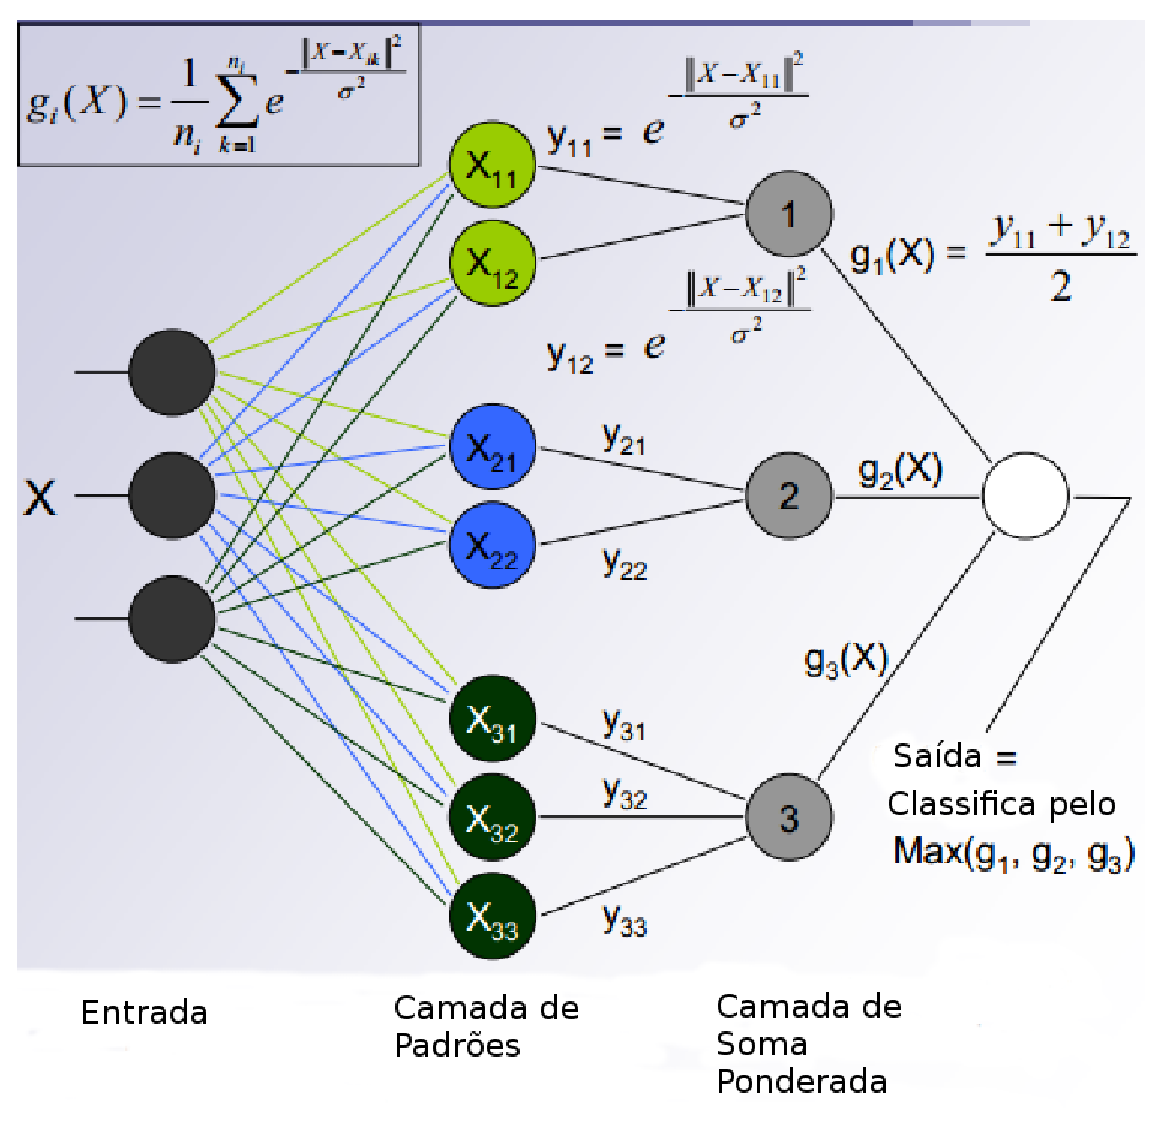
\includegraphics[scale=0.7]{figuras/PNN.eps}
	\caption{Modelo arquitetural da PNN}
\end{figure}

Ela é uma rede de 3 camadas: a primeira é responsável por classificar a probabilidade de um indivíduo ser de uma determinada classe através da distância euclidiana combinada com uma curva gaussiana; a segunda é responsável por somar e fazer uma média simples dessas probabilidades de cada classe; a terceira é responsável por extrair a classe de maior probabilidade, ou seja, pegar o valor máximo dado o conjunto de classes $\textbf{g}$. O valor final de saída é a classificação do sinal de entrada.